%! alt Regular nine-sided polygon. At vertex P, side QP is extended beyond P to a point X. The interior angle QPR is marked 140 degrees and the exterior angle XPR is marked 40 degrees, and the two make a straight line.
%! after_paragraph 1
%! scale 1/30
% The shared preamble of every Kyuclid figure. pipeline/figures turns these colours into theme-aware paint,
% and refuses any other colour, so draw only with them:
%   figink (lines and labels), figaux (construction lines), figaccent (the object the argument turns on),
%   figtint and figaccenttint (light fills).
\documentclass[border=1.5pt]{standalone}
\usepackage{tkz-euclide}
\definecolor{figink}{RGB}{0,0,0}
\definecolor{figaux}{RGB}{85,85,85}
\definecolor{figaccent}{RGB}{192,57,43}
\definecolor{figtint}{RGB}{221,221,221}
\definecolor{figaccenttint}{RGB}{245,213,208}
% tkz-euclide's defaults draw circles, compasses and marks in 50% grey and fill points with a tint.
\makeatletter
\def\tkz@otherlinecolor{figink}
\def\tkz@euc@circlecolor{figink}
\def\tkz@euc@compasscolor{figink}
\def\tkz@euc@mkcolor{figink}
\def\tkz@mk@fill{figink}
\def\tkz@euc@pointfillcolor{figink}
\makeatother
\tkzSetUpLine[color=figink,line width=.7pt]
\tkzSetUpArc[color=figink,line width=.7pt]
\tkzSetUpCompass[color=figink,line width=.5pt]
\tkzSetUpPoint[color=figink,fill=figink,size=3.1pt]
\tikzset{
  every picture/.style={line cap=round,line join=round,color=figink},
  circle style/.append style={color=figink,line width=.7pt},
  aux/.style={color=figaux,line width=.45pt,dash pattern=on 2.6pt off 2pt},
  key/.style={color=figaccent,line width=1pt},
  mk/.style={color=figink,line width=.5pt},
  lbl/.style={color=figink,inner sep=2.2pt},
  len/.style={color=figink,inner sep=1.5pt,font=\small},
}

\begin{document}
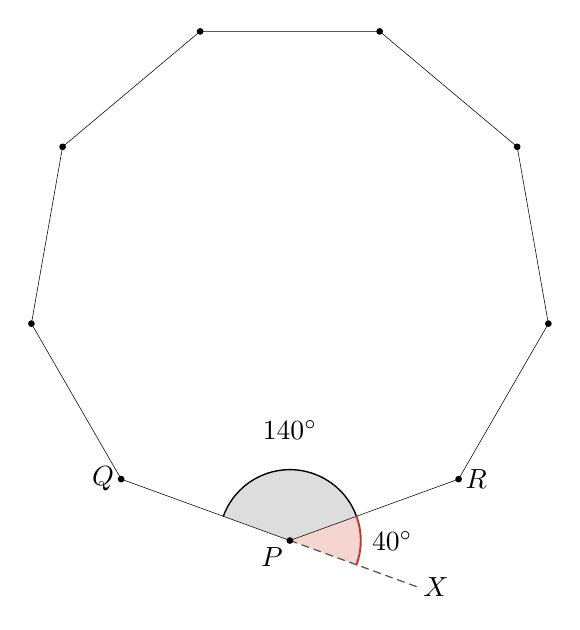
\begin{tikzpicture}
\tkzDefPoint(0.0,0.0){O} %! O = (0, 0)
\tkzDefPoint(-0.000000000000000000000000000000000000000000000000021674168,-3.3333333){P} %! P = polar(O, 100, 270)
\tkzDefPoint(2.1426254,-2.5534815){R} %! R = polar(O, 100, 310)
\tkzDefPoint(3.2826925,-0.57882726){V3} %! V3 = polar(O, 100, 350)
\tkzDefPoint(2.8867513,1.6666667){V4} %! V4 = polar(O, 100, 30)
\tkzDefPoint(1.1400671,3.1323087){V5} %! V5 = polar(O, 100, 70)
\tkzDefPoint(-1.1400671,3.1323087){V6} %! V6 = polar(O, 100, 110)
\tkzDefPoint(-2.8867513,1.6666667){V7} %! V7 = polar(O, 100, 150)
\tkzDefPoint(-3.2826925,-0.57882726){V8} %! V8 = polar(O, 100, 190)
\tkzDefPoint(-2.1426254,-2.5534815){Q} %! Q = polar(O, 100, 230)
\tkzDefPoint(1.6069690,-3.9182222){X} %! X = lerp(Q, P, 7/4)
%! fact angle(Q, P, R) == 140
%! fact angle(X, P, R) == 40
%! fact collinear(X, Q, P)
%! fact equal(dist(P, R), dist(R, V3))
%! fact equal(dist(V8, Q), dist(Q, P))
\tkzFillAngle[size=.9,color=figtint](R,P,Q)
\tkzFillAngle[size=.9,color=figaccenttint](X,P,R)
\tkzDrawPolygon(P,R,V3,V4,V5,V6,V7,V8,Q)
\tkzDrawSegment[aux](P,X)
\tkzMarkAngle[size=.9,arc=l,mark=none,mk](R,P,Q)
\tkzMarkAngle[size=.9,arc=l,mark=none,color=figaccent,line width=.7pt](X,P,R)
\tkzDrawPoints(P,R,V3,V4,V5,V6,V7,V8,Q)
\tkzLabelPoint[below left,lbl](P){$P$}
\tkzLabelPoint[right,lbl](R){$R$}
\tkzLabelPoint[left,lbl](Q){$Q$}
\tkzLabelPoint[right,lbl](X){$X$}
\tkzLabelAngle[pos=1.4](R,P,Q){$140^\circ$}
\tkzLabelAngle[pos=1.3](X,P,R){$40^\circ$}
\end{tikzpicture}
\end{document}
